\documentclass[8pt]{article}
% Эта строка — комментарий, она не будет показана в выходном файле
\usepackage{ucs}
\usepackage[utf8x]{inputenc} % Включаем поддержку UTF8
\usepackage[russian]{babel}  % Включаем пакет для поддержки русского языка
\usepackage{amsmath}
\usepackage{mathtools}
\usepackage{tabularx}
\usepackage{amssymb}
% \usepackage[dvips]{graphicx}
% \graphicspath{{noiseimages/}}
\usepackage[pdftex]{graphicx}


% Параметры страницы: 1см от правого края и 2см от остальных.


\hoffset=0mm
\voffset=0mm
\textwidth=180mm        % ширина текста
\oddsidemargin=-6.5mm   % левое поле 25.4 - 5.4 = 20 мм
\textheight=240mm       % высота текста 297 (A4) - 40
\topmargin=-15.4mm      % верхнее поле (10мм)
\headheight=5mm      % место для колонтитула
\headsep=5mm          % отступ после колонтитула
\footskip=8mm         % отступ до нижнего колонтитула


\begin{document}
    \author {Зотов Алексей 496 гр.}
    \title {Лабораторная работа 1.6 \\  Определение модуля Юнга на основе исследования деформации растяжения}
    \maketitle{}

    \textbf{Цель работы:} экспериментально получить зависимость между напряжением и деформацией (закон Гука) для одноосного растяжения. По результатам измерений вычислить модуль Юнга.

    Закон Гука для малых упругих деформаций:
    \begin{equation}
        T = E \frac{\Delta l}{l_0} = E\varepsilon
    \end{equation}
    где $T$ - сила натяжения,  $\Delta l$ — приращение длины стержня, $l_0$ — длина недеформированного стержня.
    Если принять коэффициент упругости стержня: $k=E\frac{S}{l_0}$ , то $T = k \Delta l$. \\


    \textbf{В работе используются:} прибор Лермантова(рис.1), проволока из исследуемого материала, зрительная труба со шкалой, набор грузов, микрометр, рулетка или линейка.

    \begin{center} 
        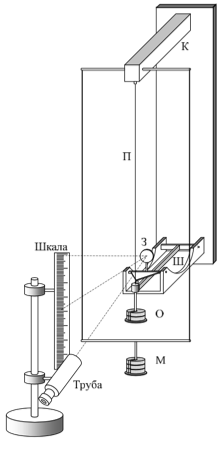
\includegraphics[width=1.0in,height=1.5in]{tool.png} \\ Рис. 1: Экспериментальная установка.
    \end{center}

    \textbf{Ход работы:}\\
    \begin{enumerate}
    \item 
        Диаметр проволоки $d = 0.46$ $mm$ \\
        Площадь поперечного сечения $S = \frac{\pi d^2}{4} \approx 0.17$ $\text{мм}^2$\\ 
    \item 
        Измеренная длина проволоки $l_0 = 177.0 \pm 0.5$ см
    \item 
        Длина рычага $r = 13$ мм \\
        Расстояние от рычага до зеркальца $h = 138.7 \pm 0.05$ см \\
        Удлинение проволки : 

        \begin{equation} \label{l}
            \Delta l = \frac{2r\Delta n}{h}
        \end{equation}

        Погрешность $\Delta l$ рассчитывается по формуле:
    
        \begin{equation} \label{dl}
        \left(\frac{\sigma_{\Delta l}}{\Delta l}\right)^2 
        = \left(\frac{\sigma_{r}}{r}\right)^2
        + \left(\frac{\sigma_{\Delta n}}{\Delta n}\right)^2
        + \left(\frac{\sigma_{h}}{h}\right)^2
        \end{equation}
    \item
        Чтобы не выйти за пределы области, где удлинение проволоки пропорционально ее натяжению, оценим максимальную величину нагрузки. Примем, что разрушающее напряжение равно $\sigma_{max} = 900$ $H/\text{мм}^2$, а допустимое напряжение не превышает $30\%$ от разрушающего.
        Тогда получим ограничение на величину нагрузки $F = \sigma S \leq 0.3 * \sigma_{max} S \approx 44.9$ Н. 
        Допустимая масса груза $m_{max} \approx 4.6 $ kg.

    \item 
        Снимем зависимость удлинения проволоки $\Delta l$ (по формуле \eqref{l})  от величины нагрузки :
    
    
    \begin{center}
    \begin{tabular}{|c|c|c|c|c|c|c|c|c|c|c|c|}
        \hline
        \textbf{$m$,г} & 0 & 498 & 992 & 1455 & 1948 & 2442 & 1948 & 1455 & 992 & 498 & 0 \\
        \hline
        \textbf{$n,$ дел} & 53.3 & 47.4 & 41.9 & 36.2 & 31.1 & 26.4 & 31.1 & 35.8 & 41.6 & 47.2 & 53.2 \\
        \hline
        \textbf{$\Delta l,$ мм} & 0 & 0.13 & 0.25 & 0.36 & 0.48 & 0.58 & 0.48 & 0.37 & 0.25 & 0.13 & 0.002\\
        \hline
    \end{tabular}
    \end{center}

    \begin{center}
    \begin{tabular}{|c|c|c|c|c|c|c|c|c|c|c|c|}
        \hline
        \textbf{$m$,г} & 0 & 498 & 992 & 1455 & 1948 & 2442 & 1948 & 1455 & 992 & 498 & 0 \\
        \hline
        \textbf{$n,$ дел} & 53.2 & 47.3 & 41.6 & 36.8 & 31.2 & 26.9 & 30.9 & 35.7 & 41.5 & 47.3 & 53.2 \\
        \hline
        \textbf{$\Delta l,$ мм} & 0 & 0.13 & 0.25 & 0.35 & 0.47 & 0.57 & 0.48 & 0.38 & 0.25 & 0.13 & 0\\
        \hline
    \end{tabular}
    \end{center}

    \begin{center}
    \begin{tabular}{|c|c|c|c|c|c|c|}
        \hline
        \textbf{$m$,г} & 498 & 992 & 1455 & 1948 & 2442\\
        \textbf{$\Delta l_{cp},$ мм} & 0.13 &  0.25  & 0.365 & 0.475 & 0.57 \\
        \hline
    \end{tabular}
    \end{center}

    \item Построим график зависимости $\Delta l(P)$ , где $P = mg$ - нагрузка
    
    \begin{center} 
        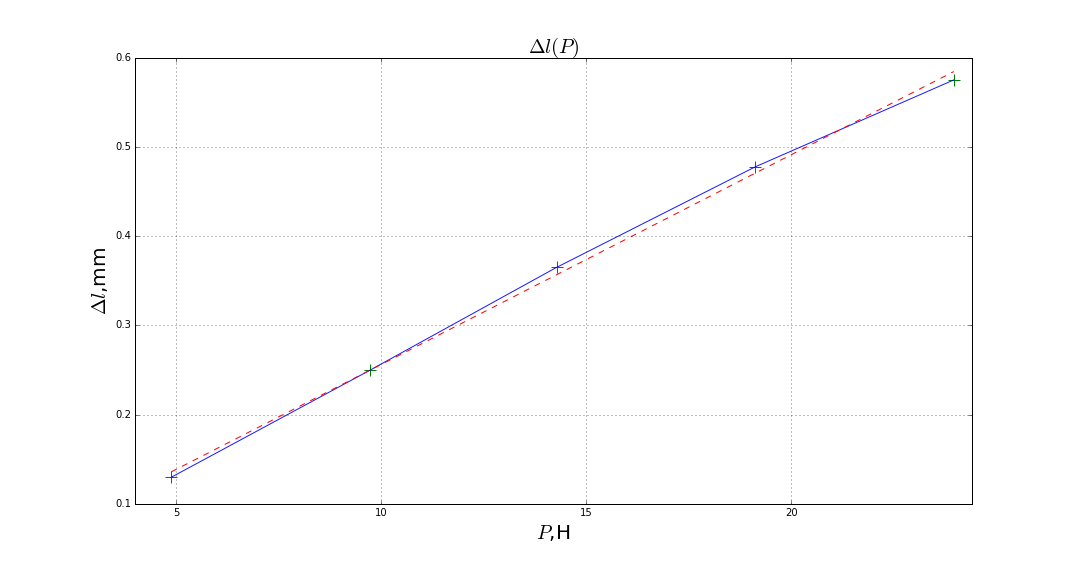
\includegraphics[width=4.5in]{graph.png} 
    \end{center}

    $y = ax + b$ , $a \approx 0.023$ , $b = 0.0234$ , $\sigma_a = 0.0005$ , $\sigma_b = 0.003$\\
    Тогда жесткость проволоки $k = \frac{P}{\Delta l} \approx \frac{1}{a} \approx 43 $ Н/мм , 
    $\sigma_k \approx \frac{1}{a^2} \sigma_a \approx 1$ Н/мм
    \item
    Найдем модуль Юнга:
    \begin{equation}
        E = \frac{kl_0}{S} = 448 \text{ГПа} 
    \end{equation}

    Оценим погрешность модуля Юнга:
    
    $$\left(\frac{\sigma_{E}}{E}\right)^2 
    = \left(\frac{\sigma_{k}}{k}\right)^2
    + \left(\frac{\sigma_{l_0}}{l_0}\right)^2
    + \left(\frac{\sigma_{S}}{S}\right)^2 \approx E \left(\frac{\sigma_{k}}{k}\right)
    \quad \Rightarrow \quad
    \sigma_{E} = 10 \text{ГПа}$$

    Наиболее близкое значение к модулю Юнга для вольфрама $E_w = 415$ Гпа.
    \end{enumerate}
    
\end{document}